\documentclass[11pt,a4paper]{article}

% Packages
\usepackage[utf8]{inputenc}
\usepackage[T1]{fontenc}
\usepackage{graphicx}
\usepackage{booktabs}
\usepackage{amsmath}
\usepackage{amssymb}
\usepackage{hyperref}
\usepackage{xcolor}
\usepackage{listings}
\usepackage{geometry}
\usepackage{float}
\usepackage{caption}
\usepackage{subcaption}
\usepackage{enumitem}
\usepackage{multicol}
\usepackage{tikz}
\usetikzlibrary{positioning, arrows.meta, shapes.geometric, shapes.misc, fit, calc, decorations.pathmorphing, backgrounds}

\geometry{margin=1in}

% Image path for Overleaf
\graphicspath{{overleaf_assets/}}

% Hyperref settings
\hypersetup{
    colorlinks=true,
    linkcolor=blue,
    filecolor=magenta,
    urlcolor=cyan,
    citecolor=blue
}

% Code listing settings
\lstset{
    basicstyle=\ttfamily\small,
    breaklines=true,
    frame=single,
    backgroundcolor=\color{gray!10}
}

% Title
\title{\textbf{Epsilon: An Autonomous Research Engine with Epistemic Integrity for Scientific Discovery}}
\author{Ritvik Jhawar \\ Independent Researcher \\ \texttt{jhawaritvik@gmail.com}}
\date{February 2026}

\begin{document}

\maketitle

% ============================================================
% ABSTRACT
% ============================================================
\begin{abstract}
The automation of scientific research presents unique challenges in maintaining methodological rigor while enabling autonomous discovery. We present \textbf{Epsilon}, a multi-agent autonomous research engine that conducts end-to-end scientific investigations, from hypothesis generation through statistical validation, without human intervention. At its core, Epsilon introduces an \textbf{epistemic integrity architecture} that enforces strict separation between the Design Agent (the ``scientist'') and the Evaluation Agent (the ``statistician''). This architectural constraint makes several common p-hacking strategies \cite{simmons2011false} structurally infeasible. Our self-correcting feedback loop enables iterative refinement when experiments fail, while a three-tier memory system (Evidence, Knowledge, Run Memory) facilitates cross-run learning and complete auditability. We evaluate Epsilon on MLAgentBench-derived tasks spanning tabular classification, natural language processing, and hyperparameter optimization. Our goal is not to outperform existing MLAgentBench agents, but to demonstrate that autonomous agents can meet benchmark targets while adhering to strict methodological constraints.

\vspace{0.5em}
\noindent\textbf{Keywords:} Autonomous Research, AI Agents, Epistemic Integrity, Multi-Agent Systems, Scientific Discovery, MLAgentBench
\end{abstract}

% ============================================================
% INTRODUCTION
% ============================================================
\section{Introduction}

The promise of artificial intelligence goes beyond automating routine tasks; it extends to automating discovery itself. Recent advances in large language models (LLMs) have made it possible for AI systems to write code, analyze data, and generate hypotheses \cite{brown2020language}. But moving from AI-assisted research to truly autonomous scientific discovery means tackling fundamental challenges around maintaining scientific rigor without human oversight.

Current approaches to AI-driven research face three critical limitations:

\begin{enumerate}
    \item \textbf{Confirmation Bias}: When the same system both designs experiments and evaluates the results, it can unconsciously (or algorithmically) favor positive outcomes. This leads to inflated success rates and findings that do not reproduce \cite{ioannidis2005why}.
    
    \item \textbf{Lack of Self-Correction}: Most automated research pipelines fall apart when the initial approach does not work, with no mechanism for iterative refinement.
    
    \item \textbf{Missing Audit Trails}: Without comprehensive logging of all decisions and iterations, automated research becomes a black box, undermining reproducibility.
\end{enumerate}

We introduce \textbf{Epsilon}, an autonomous research engine built to address these limitations through architectural innovations rather than prompt engineering alone. Our key contributions are:

\begin{itemize}
    \item \textbf{Epistemic Integrity by Design}: Strict separation between experiment design and result evaluation, enforcing structural constraints that make several common p-hacking strategies \cite{simmons2011false} infeasible.
    
    \item \textbf{Self-Correcting Feedback Loop}: A structured iteration mechanism that learns from failures and refines experimental approaches.
    
    \item \textbf{Three-Tier Memory Architecture}: Persistent storage of evidence, crystallized knowledge, and complete run audits enabling cross-run learning.
    
    \item \textbf{Statistical Rigor}: Built-in support for appropriate statistical tests including Nadeau-Bengio corrected t-tests \cite{nadeau2003inference} for resampled data.
\end{itemize}

% ============================================================
% SYSTEM ARCHITECTURE
% ============================================================
\section{System Architecture}

Epsilon uses a multi-agent architecture orchestrated by a central Controller. Each agent has a specialized role with restricted tool access, which enforces separation of concerns at the system level.

\subsection{High-Level Overview}

\begin{figure}[H]
\centering
\resizebox{\textwidth}{!}{%
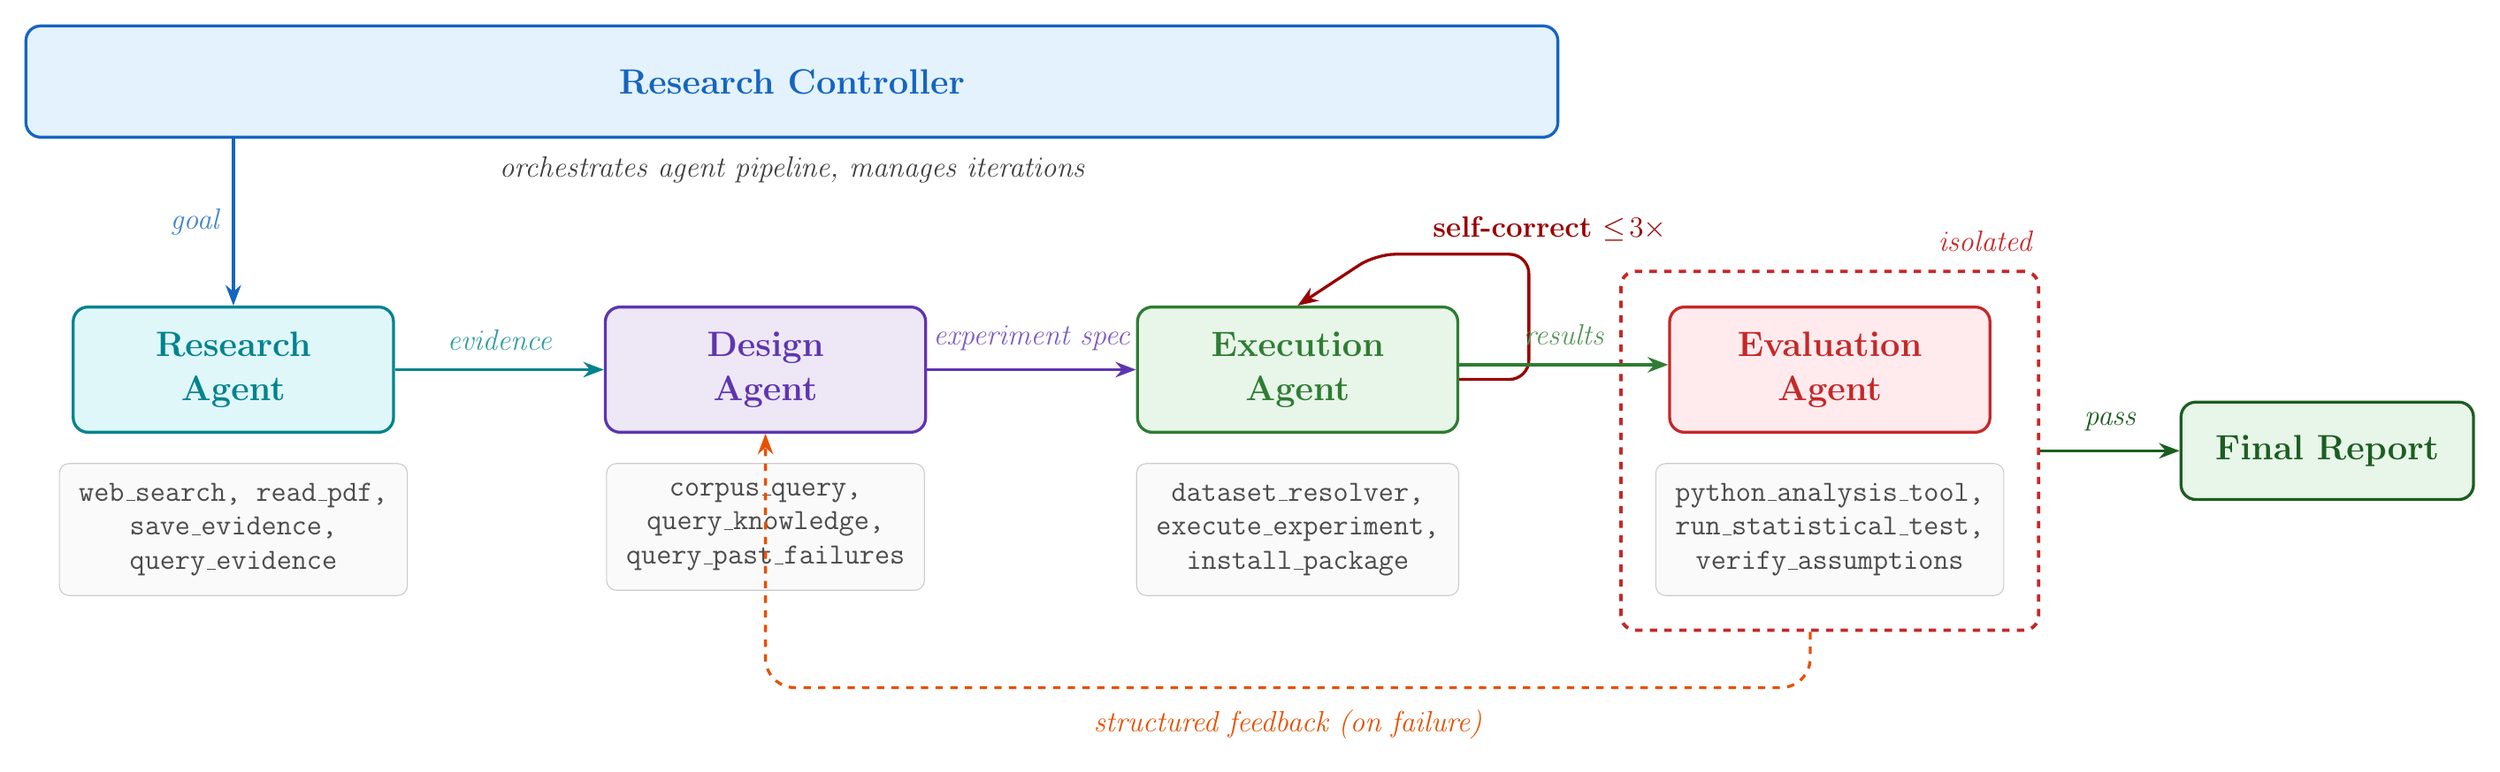
\begin{tikzpicture}[
    >=Stealth,
    node distance=1.8cm and 3.0cm,
]

% ── Colors ──
\definecolor{ctrlborder}{HTML}{1565C0}
\definecolor{ctrlfill}{HTML}{E3F2FD}
\definecolor{resborder}{HTML}{00838F}
\definecolor{resfill}{HTML}{E0F7FA}
\definecolor{desborder}{HTML}{5E35B1}
\definecolor{desfill}{HTML}{EDE7F6}
\definecolor{execborder}{HTML}{2E7D32}
\definecolor{execfill}{HTML}{E8F5E9}
\definecolor{evalborder}{HTML}{C62828}
\definecolor{evalfill}{HTML}{FFEBEE}
\definecolor{feedbackcolor}{HTML}{E65100}
\definecolor{successcolor}{HTML}{1B5E20}

% ══════════════════════════════════════════════
% ROW 1: Controller
% ══════════════════════════════════════════════
\node[rectangle, rounded corners=6pt, draw=ctrlborder, fill=ctrlfill,
    minimum width=22cm, minimum height=1.6cm,
    font=\Large\bfseries, text=ctrlborder, line width=1.2pt] (ctrl) {Research Controller};
\node[font=\large\itshape, text=gray!50!black, below=4pt of ctrl]
    (ctrlsub) {orchestrates agent pipeline, manages iterations};

% ══════════════════════════════════════════════
% ROW 2: Four agents
% ══════════════════════════════════════════════
\node[rectangle, rounded corners=6pt, draw=resborder, fill=resfill,
    minimum width=4.6cm, minimum height=1.8cm,
    font=\Large\bfseries, text=resborder, line width=1.2pt, align=center,
    below=2.4cm of ctrl.south west, anchor=north, xshift=3cm] (research) {Research\\Agent};

\node[rectangle, rounded corners=6pt, draw=desborder, fill=desfill,
    minimum width=4.6cm, minimum height=1.8cm,
    font=\Large\bfseries, text=desborder, line width=1.2pt, align=center,
    right=3.0cm of research] (design) {Design\\Agent};

\node[rectangle, rounded corners=6pt, draw=execborder, fill=execfill,
    minimum width=4.6cm, minimum height=1.8cm,
    font=\Large\bfseries, text=execborder, line width=1.2pt, align=center,
    right=3.0cm of design] (execute) {Execution\\Agent};

\node[rectangle, rounded corners=6pt, draw=evalborder, fill=evalfill,
    minimum width=4.6cm, minimum height=1.8cm,
    font=\Large\bfseries, text=evalborder, line width=1.2pt, align=center,
    right=3.0cm of execute] (evaluate) {Evaluation\\Agent};

% ══════════════════════════════════════════════
% ROW 3: Tool boxes (below each agent)
% ══════════════════════════════════════════════
\node[rectangle, rounded corners=4pt, draw=gray!40, fill=gray!4,
    font=\ttfamily\large, text=gray!60!black, inner sep=8pt, align=center,
    below=12pt of research] (rt) {web\_search, read\_pdf,\\save\_evidence,\\query\_evidence};

\node[rectangle, rounded corners=4pt, draw=gray!40, fill=gray!4,
    font=\ttfamily\large, text=gray!60!black, inner sep=8pt, align=center,
    below=12pt of design] (dt) {corpus\_query,\\query\_knowledge,\\query\_past\_failures};

\node[rectangle, rounded corners=4pt, draw=gray!40, fill=gray!4,
    font=\ttfamily\large, text=gray!60!black, inner sep=8pt, align=center,
    below=12pt of execute] (et) {dataset\_resolver,\\execute\_experiment,\\install\_package};

\node[rectangle, rounded corners=4pt, draw=gray!40, fill=gray!4,
    font=\ttfamily\large, text=gray!60!black, inner sep=8pt, align=center,
    below=12pt of evaluate] (vt) {python\_analysis\_tool,\\run\_statistical\_test,\\verify\_assumptions};

% ══════════════════════════════════════════════
% Isolation box around Evaluation Agent + tools
% ══════════════════════════════════════════════
\node[rectangle, rounded corners=6pt, draw=evalborder, dashed,
    line width=1.4pt, inner sep=14pt, fit=(evaluate)(vt)] (isobox) {};
\node[font=\large\itshape, text=evalborder, anchor=south east]
    at ([yshift=4pt]isobox.north east) {isolated};

% ══════════════════════════════════════════════
% Self-correction loop (above Execution Agent)
% ══════════════════════════════════════════════
\draw[->, very thick, red!60!black, rounded corners=8pt]
    ([yshift=-4pt]execute.east) -- ++(1.0,0) -- ++(0,1.8) -- ++(-2.2,0) -- (execute.north);
\node[font=\large\bfseries, text=red!60!black, fill=white, inner sep=3pt,
    rounded corners=3pt]
    at ([xshift=1.3cm, yshift=1.1cm]execute.north east) {self-correct $\leq\!3\times$};

% ══════════════════════════════════════════════
% Flow arrows: Controller -> Agents -> Agents
% ══════════════════════════════════════════════
\draw[->, very thick, ctrlborder] (ctrl.south -| research.north) -- (research.north)
    node[midway, left=2pt, font=\large\itshape, text=ctrlborder!80] {goal};
\draw[->, very thick, resborder] (research.east) -- (design.west)
    node[midway, above=4pt, font=\large\itshape, text=resborder!80] {evidence};
\draw[->, very thick, desborder] (design.east) -- (execute.west)
    node[midway, above=4pt, font=\large\itshape, text=desborder!80] {experiment spec};
\draw[->, very thick, execborder] ([yshift=2pt]execute.east) -- ([yshift=2pt]evaluate.west)
    node[midway, above=4pt, font=\large\itshape, text=execborder!80] {results};

% ══════════════════════════════════════════════
% Success path: Evaluation -> Final Report (to the right)
% ══════════════════════════════════════════════
\node[rectangle, rounded corners=6pt, draw=successcolor, fill=execfill,
    minimum width=4.2cm, minimum height=1.4cm,
    font=\Large\bfseries, text=successcolor, line width=1.2pt,
    right=2.0cm of isobox] (report) {Final Report};
\draw[->, very thick, successcolor] (isobox.east) -- (report.west)
    node[midway, above=4pt, font=\large\itshape, text=successcolor] {pass};

% ══════════════════════════════════════════════
% Feedback arc (on failure, back to Design Agent)
% ══════════════════════════════════════════════
\draw[->, very thick, feedbackcolor, dashed, rounded corners=12pt]
    ([xshift=-8pt]isobox.south) -- ++(0,-0.8) -| (design.south)
    node[pos=0.25, below=5pt, font=\large\itshape, text=feedbackcolor] {structured feedback (on failure)};

\end{tikzpicture}%
}% end resizebox
\caption{Agent architecture with isolated evaluation. The Evaluation Agent (dashed border) cannot modify hypotheses or re-run experiments, ensuring unbiased validation. The Execution Agent retries failed code up to three times before escalating to the outer loop.}
\label{fig:architecture}
\end{figure}

\subsection{Agent Responsibilities}

\begin{table}[H]
\centering
\begin{tabular}{@{}lll@{}}
\toprule
\textbf{Agent} & \textbf{Role} & \textbf{Primary Tools} \\
\midrule
Research Agent & Literature review & \texttt{web\_search}, \texttt{read\_pdf}, \texttt{save\_evidence}, \texttt{query\_evidence} \\
Design Agent & Hypothesis formulation & \texttt{corpus\_query}, \texttt{query\_knowledge}, \texttt{query\_past\_failures} \\
Execution Agent & Code generation \& execution & \texttt{dataset\_resolver}, \texttt{execute\_experiment}, \texttt{install\_package} \\
Evaluation Agent & Statistical validation & \texttt{python\_analysis\_tool}, \texttt{run\_statistical\_test}, \texttt{verify\_assumptions} \\
\bottomrule
\end{tabular}
\caption{Agent Responsibilities and Tool Access. Each agent's tool set is restricted by design; e.g., the Evaluation Agent has no design or execution tools.}
\label{tab:agents}
\end{table}

\subsubsection*{Tool Descriptions}

Each agent is given a small, purpose-specific set of tools. The tool boundaries are enforced at the framework level: an agent simply cannot call a tool that is not in its toolset.

\textbf{Research Agent Tools.}

\begin{itemize}
    \item \texttt{web\_search(query)}: Searches the web using the Tavily API and returns a summary of results. This is the primary mechanism for literature discovery.
    \item \texttt{read\_pdf(url)}: Downloads a PDF from a URL, extracts the full text, and returns it for analysis. Used for reading academic papers found during search.
    \item \texttt{save\_evidence(source\_type, source\_url, extracted\_claim, \ldots)}: Persists a specific research finding to Evidence Memory. Each entry includes the source URL, the extracted claim, supporting text, and a confidence level, ensuring full provenance tracking.
    \item \texttt{query\_evidence(query)}: Queries the Evidence Memory for previously saved findings related to a topic. The agent is instructed to call this before starting new searches to avoid redundant work (read-before-write deduplication).
\end{itemize}

\textbf{Design Agent Tools.}

\begin{itemize}
    \item \texttt{corpus\_query(query)}: Searches the global Evidence Memory for research findings saved by the Research Agent. This gives the Design Agent access to the evidence base without needing its own search capabilities.
    \item \texttt{query\_knowledge(query)}: Retrieves validated, crystallized knowledge from Knowledge Memory. These are conclusions from previous runs that passed statistical validation, giving the agent access to established facts.
    \item \texttt{query\_past\_failures(query)}: Retrieves records of past failed iterations from Run Memory, automatically filtered for failed runs. This lets the Design Agent avoid repeating approaches that previously did not work.
\end{itemize}

\textbf{Execution Agent Tools.}

\begin{itemize}
    \item \texttt{dataset\_resolver(data\_modality, dataset\_requirements)}: Resolves data acquisition from explicit design signals. Given a modality (e.g., ``tabular'', ``image'') and requirements (e.g., dataset name, feature count), it returns structured metadata describing how to load the dataset. Supports scikit-learn, HuggingFace, and procedural generation sources. The Execution Agent is bound to use the resolved dataset exactly as returned.
    \item \texttt{execute\_experiment(code)}: Saves the provided Python code to \texttt{run\_experiment.py} and executes it, capturing stdout, stderr, and return status. Execution can occur inside a Docker container (for sandboxing) or locally via subprocess.
    \item \texttt{install\_package(package\_name)}: Installs a Python package into the current environment using pip. Used only when the agent encounters a \texttt{ModuleNotFoundError} during experiment execution.
\end{itemize}

\textbf{Evaluation Agent Tools.}

\begin{itemize}
    \item \texttt{python\_analysis\_tool(code)}: Executes arbitrary Python code in a pre-configured environment with \texttt{pandas}, \texttt{numpy}, and \texttt{scipy.stats} already imported. The Evaluation Agent uses this to load raw result files, compute summary statistics, and extract metrics directly from data. This is the primary mechanism through which the agent reads experimental output.
    \item \texttt{run\_statistical\_test(test\_name, data\_a, data\_b, alpha, alternative)}: Executes a specific statistical test on the provided data arrays. Supported tests include independent and paired t-tests, Mann-Whitney U, Wilcoxon signed-rank, and Shapiro-Wilk. Returns the test statistic, p-value, and a decision (reject or fail to reject $H_0$).
    \item \texttt{verify\_assumptions(check\_type, data)}: Verifies statistical assumptions before running parametric tests. Currently supports normality checking via the Shapiro-Wilk test. If the assumption fails, the agent falls back to a non-parametric alternative.
\end{itemize}

Notably, the Execution Agent implements an internal \textbf{self-correction loop}: when code execution fails, the agent diagnoses the error from logs, regenerates the code, and re-executes, repeating this cycle up to three times. This includes automatic dependency installation via \texttt{install\_package} when missing imports are detected. The reason for this inner loop is practical: LLM-generated code frequently hits runtime errors (missing imports, type mismatches, API changes), and sending every such mechanical failure through the full epistemic loop would waste time and compute. By letting the Execution Agent handle its own fixes locally, the outer loop stays focused on genuine scientific revisions from the Evaluation Agent.

\subsection{The Epistemic Loop}

The core workflow follows a structured loop with explicit failure handling. At each iteration, the Research Agent gathers evidence from the literature, the Design Agent formulates a hypothesis and experiment specification, the Execution Agent runs the code, and the Evaluation Agent independently validates the results. If the Evaluation Agent determines the results are not statistically robust, it sends structured feedback (including the failure type, failing metric, and a suggested revision) to the Design Agent, which re-designs the experiment. This loop repeats up to $N$ iterations (default $N{=}5$). If the evaluation passes, the validated conclusion is crystallized into long-term knowledge and the system produces a final report.

\subsection{Memory Architecture}

Epsilon implements a three-tier memory system backed by Supabase:

\begin{figure}[H]
\centering
\resizebox{0.92\textwidth}{!}{%
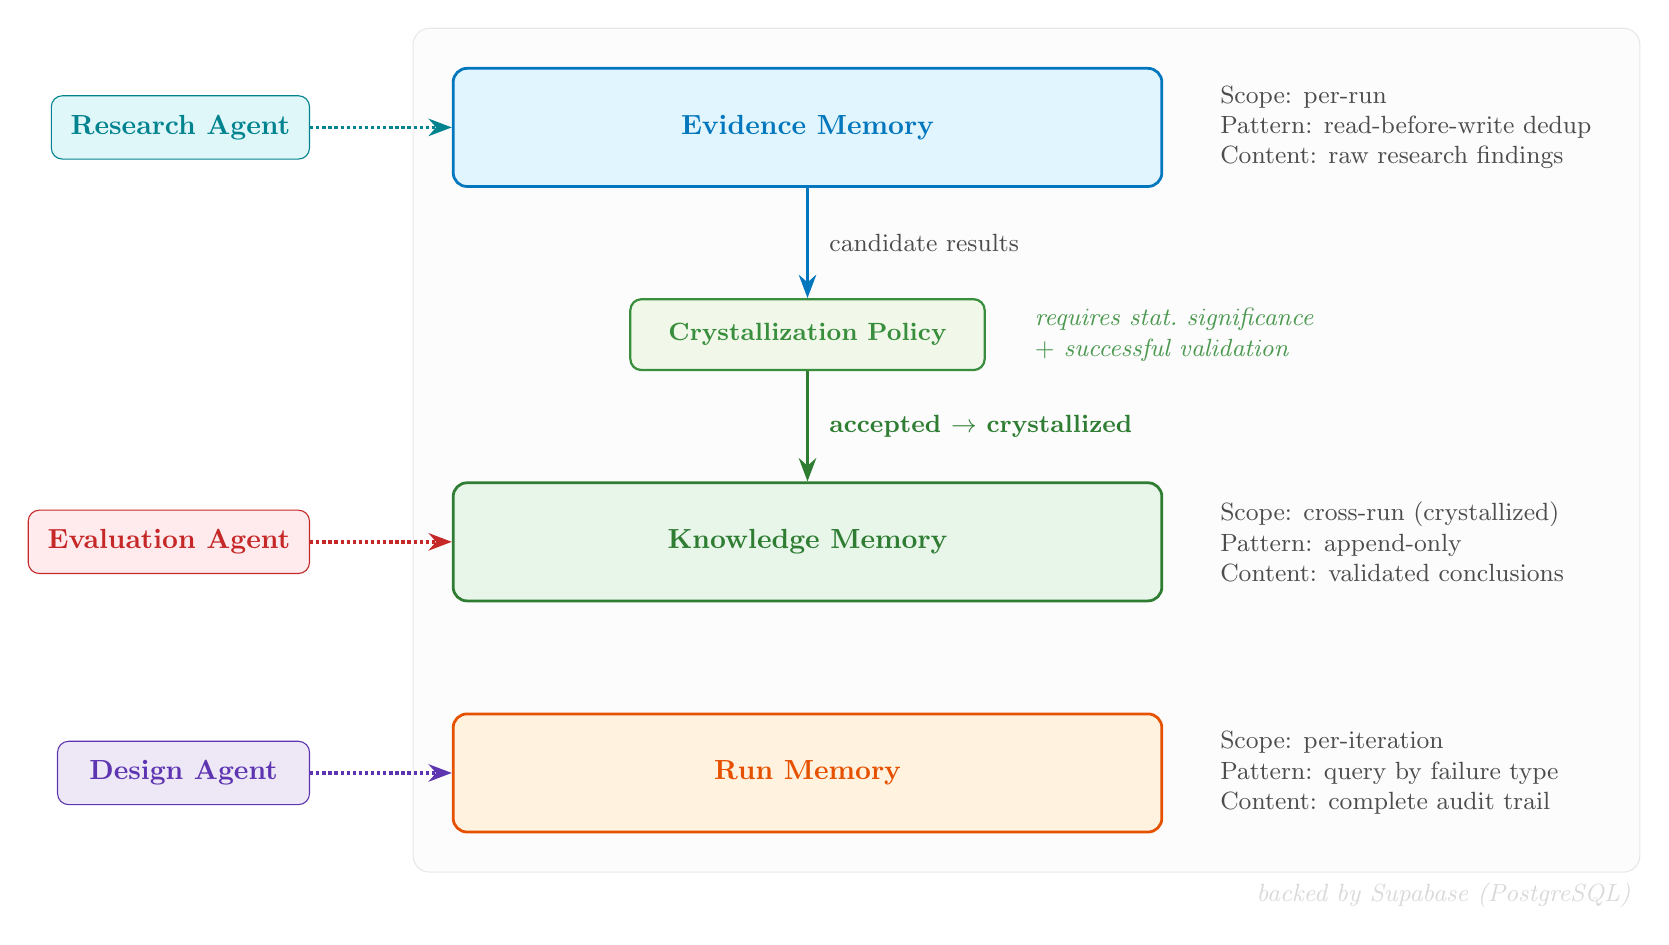
\begin{tikzpicture}[
    >=Stealth,
    node distance=1.2cm,
]

% ── Colors ──
\definecolor{evborder}{HTML}{0277BD}
\definecolor{evfill}{HTML}{E1F5FE}
\definecolor{knborder}{HTML}{2E7D32}
\definecolor{knfill}{HTML}{E8F5E9}
\definecolor{rmborder}{HTML}{E65100}
\definecolor{rmfill}{HTML}{FFF3E0}
\definecolor{gateborder}{HTML}{388E3C}
\definecolor{gatefill}{HTML}{F1F8E9}
\definecolor{resborder}{HTML}{00838F}
\definecolor{resfill}{HTML}{E0F7FA}
\definecolor{evalborder}{HTML}{C62828}
\definecolor{evalfill}{HTML}{FFEBEE}
\definecolor{desborder}{HTML}{5E35B1}
\definecolor{desfill}{HTML}{EDE7F6}

% ══════════════════════════════════════════════
% TIER 1: Evidence Memory
% ══════════════════════════════════════════════
\node[rectangle, rounded corners=5pt, draw=evborder, fill=evfill,
    minimum width=9cm, minimum height=1.5cm,
    font=\normalsize\bfseries, text=evborder, line width=1pt]
    (evidence) {Evidence Memory};
\node[font=\small, text=gray!60!black, right=0.6cm of evidence.east, anchor=west,
    align=left] (evdetail) {
    Scope: per-run\\
    Pattern: read-before-write dedup\\
    Content: raw research findings
};

% ══════════════════════════════════════════════
% Crystallization gate (between Evidence and Knowledge)
% ══════════════════════════════════════════════
\node[rectangle, rounded corners=4pt, draw=gateborder, fill=gatefill,
    minimum width=4.5cm, minimum height=0.9cm,
    font=\small\bfseries, text=gateborder, line width=0.8pt,
    below=1.4cm of evidence] (gate) {Crystallization Policy};

% Gate description: placed to the RIGHT of the gate
\node[font=\small\itshape, text=gateborder!90,
    anchor=west, align=left]
    at ([xshift=0.5cm]gate.east) (gatedesc) {requires stat.\ significance\\$+$ successful validation};

% ══════════════════════════════════════════════
% TIER 2: Knowledge Memory
% ══════════════════════════════════════════════
\node[rectangle, rounded corners=5pt, draw=knborder, fill=knfill,
    minimum width=9cm, minimum height=1.5cm,
    font=\normalsize\bfseries, text=knborder, line width=1pt,
    below=1.4cm of gate] (knowledge) {Knowledge Memory};
\node[font=\small, text=gray!60!black, right=0.6cm of knowledge.east, anchor=west,
    align=left] (kndetail) {
    Scope: cross-run (crystallized)\\
    Pattern: append-only\\
    Content: validated conclusions
};

% ══════════════════════════════════════════════
% TIER 3: Run Memory
% ══════════════════════════════════════════════
\node[rectangle, rounded corners=5pt, draw=rmborder, fill=rmfill,
    minimum width=9cm, minimum height=1.5cm,
    font=\normalsize\bfseries, text=rmborder, line width=1pt,
    below=1.4cm of knowledge] (runmem) {Run Memory};
\node[font=\small, text=gray!60!black, right=0.6cm of runmem.east, anchor=west,
    align=left] (rmdetail) {
    Scope: per-iteration\\
    Pattern: query by failure type\\
    Content: complete audit trail
};

% ══════════════════════════════════════════════
% Arrows between tiers
% ══════════════════════════════════════════════
\draw[->, very thick, evborder] (evidence) -- (gate)
    node[midway, right=4pt, font=\small, text=gray!60!black] {candidate results};
\draw[->, very thick, knborder] (gate) -- (knowledge)
    node[midway, right=4pt, font=\small\bfseries, text=knborder] {accepted $\rightarrow$ crystallized};


% ══════════════════════════════════════════════
% Agent access labels (left side)
% ══════════════════════════════════════════════
\node[rectangle, rounded corners=4pt, draw=resborder, fill=resfill,
    font=\normalsize\bfseries, text=resborder, inner sep=7pt, minimum width=3.2cm,
    left=1.8cm of evidence] (ra) {Research Agent};
\draw[->, densely dotted, resborder, very thick] (ra) -- (evidence);

\node[rectangle, rounded corners=4pt, draw=evalborder, fill=evalfill,
    font=\normalsize\bfseries, text=evalborder, inner sep=7pt, minimum width=3.2cm,
    left=1.8cm of knowledge] (ea) {Evaluation Agent};
\draw[->, densely dotted, evalborder, very thick] (ea) -- (knowledge);

\node[rectangle, rounded corners=4pt, draw=desborder, fill=desfill,
    font=\normalsize\bfseries, text=desborder, inner sep=7pt, minimum width=3.2cm,
    left=1.8cm of runmem] (da) {Design Agent};
\draw[->, densely dotted, desborder, very thick] (da) -- (runmem);

% ══════════════════════════════════════════════
% Backend enclosure
% ══════════════════════════════════════════════
\begin{scope}[on background layer]
\node[rectangle, rounded corners=6pt, draw=gray!18, fill=gray!2,
    fit=(evidence)(knowledge)(runmem)(evdetail)(kndetail)(rmdetail)(gate), inner sep=14pt] (backend) {};
\end{scope}
\node[font=\small\itshape, text=gray!30, anchor=north east]
    at (backend.south east) {backed by Supabase (PostgreSQL)};

\end{tikzpicture}%
}% end resizebox
\caption{Three-Tier Memory Architecture. Evidence is crystallized into Knowledge only when the Crystallization Policy is satisfied (statistical significance and successful validation), preventing pollution from failed experiments.}
\label{fig:memory}
\end{figure}

\begin{table}[H]
\centering
\begin{tabular}{@{}llll@{}}
\toprule
\textbf{Memory Type} & \textbf{Purpose} & \textbf{Persistence} & \textbf{Access Pattern} \\
\midrule
Evidence Memory & Raw research findings & Per-run & Read-before-write dedup \\
Knowledge Memory & Validated conclusions & Crystallized & Append-only \\
Run Memory & Complete audit trail & Per-iteration & Query by failure type \\
\bottomrule
\end{tabular}
\caption{Three-Tier Memory Architecture}
\label{tab:memory}
\end{table}

\textbf{Knowledge Crystallization}: Only results that meet strict criteria (statistical significance, successful validation) get promoted to Knowledge Memory. This prevents pollution from failed experiments.

% ============================================================
% THREAT MODEL
% ============================================================
\section{Threat Model and Failure Modes}

To be clear about what Epsilon can and cannot guarantee, we spell out the threats it is designed to handle and the ones it does not claim to mitigate.

\subsection{Threat Model}

\begin{table}[H]
\centering
\begin{tabular}{@{}lll@{}}
\toprule
\textbf{Threat} & \textbf{Mitigated?} & \textbf{Mechanism} \\
\midrule
Metric switching after results & Yes & Pre-specified evaluation plan \\
Hypothesis rewriting post-hoc & Yes & Role separation (Design $\not\rightarrow$ Eval) \\
Optional stopping / early termination & Yes & Fixed iteration budget \\
Selective reporting of runs & Yes & Complete audit trail in Run Memory \\
\midrule
Poor initial hypothesis quality & No & Depends on LLM capabilities \\
Dataset bias / selection effects & No & External to system scope \\
Adversarial prompt injection & No & Not in current threat model \\
\bottomrule
\end{tabular}
\caption{Explicit Threat Model: What Epsilon Does and Does Not Address}
\label{tab:threat}
\end{table}

\subsection{Why Ablation of Epistemic Separation Is Structurally Infeasible}

A natural question is whether we can isolate the benefits of epistemic separation through ablation. We argue that this is structurally infeasible, for the following reasons:

\begin{enumerate}
    \item \textbf{System Class Change}: Removing epistemic separation does not yield a ``simplified Epsilon.'' Instead, it yields a fundamentally different system that violates the threat model Epsilon is designed to address. The separation is not an optimizable component but a design constraint.
    
    \item \textbf{Clinical Trial Analogy}: Ablating role separation is comparable to ablating blinding in a clinical trial. While technically possible, the resulting system answers a different scientific question and provides incomparable evidence.
    
    \item \textbf{Capability vs. Behavior}: Epsilon's contribution is not that separated systems \textit{behave} better on benchmarks, but that they \textit{cannot} perform certain manipulations. Ablation would measure behavioral differences, not capability constraints.
\end{enumerate}

We therefore treat epistemic integrity as an architectural assumption rather than a tunable hyperparameter.

% ============================================================
% METHODOLOGY
% ============================================================
\section{Methodology}

\subsection{Epistemic Integrity Principle}

Epsilon's central design principle is the \textbf{strict separation of epistemic roles}. The Evaluation Agent does receive the experiment specification (including hypotheses and success criteria) so it can render a verdict, but it is structurally constrained:

\begin{itemize}
    \item Cannot modify experiment parameters, hypotheses, or success criteria (no design tools available)
    \item Must consume the \texttt{success\_spec} from the Design Agent blindly: it validates against pre-specified thresholds without authority to redefine metrics
    \item Reads raw data files via \texttt{python\_analysis\_tool} and applies pre-specified statistical tests
    \item Has no execution tools, so it cannot re-run experiments or alter generated code
\end{itemize}

This separation enforces \textbf{role-based access control} rather than information hiding. The Evaluation Agent knows \textit{what} to evaluate but cannot influence \textit{how} the experiment was designed or executed. This mirrors the role of a statistician in a clinical trial who knows the protocol but cannot alter the treatment assignments.

\subsection{Dataset Resolution}

The Execution Agent resolves datasets through a deterministic pipeline:

\begin{enumerate}
    \item Parse \texttt{data\_modality} from experiment specification
    \item Match against known sources (sklearn, HuggingFace, procedural generation)
    \item Return structured dataset metadata for code generation
    \item Enforce strict binding so the agent must use the resolved dataset
\end{enumerate}

\subsection{Statistical Framework}

Epsilon supports multiple statistical tests with automatic assumption verification:

\begin{itemize}
    \item \textbf{Normality Check}: Shapiro-Wilk test \cite{shapiro1965analysis} before parametric tests
    \item \textbf{Primary Tests}: Independent and paired t-tests
    \item \textbf{Fallback Tests}: Mann-Whitney U \cite{mann1947test}, Wilcoxon signed-rank \cite{wilcoxon1945individual} for non-normal data
    \item \textbf{Corrected Statistics}: Nadeau-Bengio correction \cite{nadeau2003inference} for resampled/cross-validated comparisons (applied within generated experiment code when the Design Agent specifies repeated holdout evaluation)
\end{itemize}

\subsection{Self-Correction Mechanism}

When evaluation fails, the system generates structured feedback:

\begin{lstlisting}[language=json]
{
  "outcome": "failed",
  "issue_type": "assumption_violation | design | execution",
  "rationale": "Normality assumption violated (Shapiro p=0.003)",
  "revision_directives": "Consider non-parametric test"
}
\end{lstlisting}

This feedback gets passed to the Experiment Agent for the next iteration, giving it concrete guidance for targeted refinement.

\subsection{Observed Failure Cases}

To demonstrate that Epsilon does not contort metrics to achieve success, we describe observed failure modes from our experimental runs:

\textbf{Case 1: Regression Experiment}. In an early run, the system attempted to improve RMSE using feature engineering. The Evaluation Agent correctly reported failure when the achieved RMSE ratio was 1.19 (target: $\leq$0.90). The system did not:
\begin{itemize}
    \item Switch to a different metric where results looked better
    \item Reframe the hypothesis post-hoc
    \item Selectively report a subset of folds
\end{itemize}
Instead, it logged the failure with issue type \texttt{target\_not\_met} and generated revision directives for the next iteration.

\textbf{Case 2: Assumption Validation}. During hyperparameter optimization, initial runs triggered Shapiro-Wilk violations ($p < 0.05$). Rather than proceeding with invalid parametric tests, the Evaluation Agent flagged \texttt{assumption\_violation} and the system automatically switched to non-parametric Wilcoxon analysis.

These cases demonstrate that the architecture enforces honest reporting even when results are unfavorable.

% ============================================================
% EXPERIMENTAL EVALUATION
% ============================================================
\section{Experimental Evaluation}

We evaluate Epsilon on three benchmark tasks derived from MLAgentBench, covering diverse machine learning domains. \textbf{Our goal is not to outperform existing MLAgentBench agents, but to show that autonomous agents can meet benchmark targets while adhering to strict methodological constraints.} This represents a different axis of evaluation: methodological rigor rather than raw performance.

\subsection{Tabular Classification (Adult Income)}

\textbf{Objective}: Improve classification accuracy for predicting income \textgreater\$50K using the Adult Income dataset.

\textbf{Dataset}: UCI Adult Income \cite{kohavi1996adult} (48,842 samples, 14 features)

\textbf{Experimental Setup}:
\begin{itemize}
    \item Baseline: Gradient Boosting with default parameters
    \item Enhanced: Hyperparameter-tuned Gradient Boosting (GridSearchCV)
    \item Metrics: Accuracy, Balanced Accuracy, ROC-AUC
\end{itemize}

\textbf{Results}:

\begin{table}[H]
\centering
\begin{tabular}{@{}lccc@{}}
\toprule
\textbf{Metric} & \textbf{Baseline} & \textbf{Tuned} & \textbf{Improvement} \\
\midrule
Accuracy & 86.76\% & \textbf{87.59\%} & +0.83\% \\
Balanced Accuracy & 77.58\% & \textbf{79.88\%} & +2.30\% \\
ROC-AUC & 0.921 & \textbf{0.929} & +0.008 \\
\bottomrule
\end{tabular}
\caption{Adult Income Classification Results}
\label{tab:task2}
\end{table}

\textbf{Statistical Validation}: One-sided binomial test against 78\% target yielded p-value = $6.69 \times 10^{-132}$, confirming statistically significant improvement.

\textbf{Epsilon's Approach}: The system autonomously identified that feature engineering and hyperparameter tuning would yield the largest gains. Key tuned parameters: learning\_rate=0.05, n\_estimators=300, max\_depth=5.

\begin{figure}[H]
\centering
\includegraphics[width=0.7\textwidth]{tabular_classification_results.png}
\caption{Tabular Classification: Baseline vs. Tuned Gradient Boosting performance comparison on the Adult Income dataset.}
\label{fig:tabular_results}
\end{figure}

\subsection{Text Sentiment Analysis (IMDB)}

\textbf{Objective}: Improve sentiment classification on IMDB movie reviews using TF-IDF and n-gram feature engineering.

\textbf{Dataset}: Stanford IMDB \cite{maas2011learning} (50,000 reviews, binary sentiment)

\textbf{Experimental Setup}:
\begin{itemize}
    \item Baseline: LinearSVC with unigram TF-IDF
    \item Enhanced: LinearSVC with bigrams (1,2) and negation handling
    \item Validation: 5-fold stratified cross-validation
\end{itemize}

\textbf{Results}:

\begin{table}[H]
\centering
\begin{tabular}{@{}lcc@{}}
\toprule
\textbf{Configuration} & \textbf{CV Mean Accuracy} & \textbf{Std Dev} \\
\midrule
Unigram baseline & 89.4\% & $\pm$0.3\% \\
Bigram (1,2) & 90.5\% & $\pm$0.2\% \\
\textbf{Bigram + Negation} & \textbf{90.62\%} & $\pm$0.3\% \\
\bottomrule
\end{tabular}
\caption{IMDB Sentiment Classification Results}
\label{tab:task3}
\end{table}

\textbf{Statistical Validation}: 
\begin{itemize}
    \item Paired t-test: $t=8.06$, $p=0.0006$ (one-sided)
    \item Shapiro-Wilk normality: $p=0.783$ (assumption satisfied)
    \item Wilcoxon fallback: $p=0.0009$ (corroborating evidence)
\end{itemize}

\textbf{Epsilon's Approach}: The system hypothesized that capturing negation context (``not good'' vs ``good'') would improve sentiment detection. It implemented a custom negation prefix approach combined with bigram features.

\begin{figure}[H]
\centering
\includegraphics[width=0.7\textwidth]{text_sentiment_results.png}
\caption{Text Sentiment Analysis: Accuracy comparison across TF-IDF configurations on the IMDB dataset.}
\label{fig:sentiment_results}
\end{figure}

\subsection{Hyperparameter Optimization (MNIST MLP)}

\textbf{Objective}: Demonstrate that nested cross-validation \cite{varma2006bias} hyperparameter optimization improves MLP performance on MNIST.

\textbf{Dataset}: MNIST digits \cite{lecun1998gradient} (subset for computational efficiency)

\textbf{Experimental Setup}:
\begin{itemize}
    \item Baseline: MLP with default hyperparameters (lr=0.001, batch=64, hidden=[50])
    \item Enhanced: Grid search over 27 configurations with nested CV
    \item Outer loop: 30 repeated stratified holdouts ($J=30$)
    \item Inner loop: 5-fold CV for hyperparameter selection
\end{itemize}

\textbf{Results}:

\begin{table}[H]
\centering
\begin{tabular}{@{}lccc@{}}
\toprule
\textbf{Metric} & \textbf{Baseline} & \textbf{Optimized} & \textbf{Difference} \\
\midrule
Mean Accuracy & 94.59\% & \textbf{95.35\%} & +0.76\% \\
Std Dev & 1.64\% & 1.16\% & -0.48\% \\
\bottomrule
\end{tabular}
\caption{MNIST Hyperparameter Optimization Results}
\label{tab:task5}
\end{table}

\textbf{Statistical Validation}:
\begin{itemize}
    \item Nadeau-Bengio corrected t-test: $t=1.26$, $p=0.217$ (two-sided)
    \item Wilcoxon signed-rank: $p=0.0009$ (two-sided)
    \item 95\% CI for improvement: $[-0.47\%, +1.99\%]$
\end{itemize}

We interpret the MNIST results as evidence of a potential improvement under conservative non-parametric analysis (Wilcoxon $p=0.0009$), while acknowledging that parametric corrected tests leave the result inconclusive ($p=0.217$). This kind of transparency reflects Epsilon's commitment to honest statistical reporting over outcome-driven interpretation.

\textbf{Most Frequently Selected Configuration}: batch\_size=32, hidden\_layer\_sizes=[100], learning\_rate\_init=0.01 (selected in 10/30 outer repeats)

\begin{figure}[H]
\centering
\includegraphics[width=0.7\textwidth]{hyperparameter_optimization_results.png}
\caption{Hyperparameter Optimization: MLP accuracy distribution across 30 repeated holdouts comparing default vs. optimized hyperparameters on MNIST.}
\label{fig:hyperparam_results}
\end{figure}

\subsection{Summary of Results}

\begin{table}[H]
\centering
\begin{tabular}{@{}lllll@{}}
\toprule
\textbf{Task} & \textbf{Domain} & \textbf{Target} & \textbf{Achieved} & \textbf{Statistical Evidence} \\
\midrule
Tabular Classification & Structured Data & $\geq$78\% & 87.59\% & Binomial $p=6.7\times10^{-132}$ \\
Text Sentiment & NLP & $\geq$87\% & 90.62\% & Paired t $p=0.0006$ \\
Hyperparameter Opt. & AutoML & Improvement & +0.76\% & Wilcoxon $p=0.0009$ \\
\bottomrule
\end{tabular}
\caption{Summary of Experimental Results}
\label{tab:summary}
\end{table}

% ============================================================
% RELATED WORK
% ============================================================
\section{Related Work}

\subsection{AI Research Agents}

\textbf{MLAgentBench} \cite{huang2024mlagentbench} provides a benchmark for evaluating AI agents on machine learning research tasks. Our work extends this by implementing a complete autonomous pipeline with epistemic safeguards.

\textbf{The AI Scientist} \cite{lu2024aiscientist} demonstrated end-to-end paper generation from idea to manuscript. While impressive, it lacks the structural separation between design and evaluation that prevents confirmation bias.

\subsection{AutoML Systems}

AutoML systems (Auto-sklearn \cite{feurer2015automl}, TPOT \cite{olson2016tpot}, H2O \cite{ledell2020h2o}) focus on model selection and hyperparameter optimization but lack the higher-level research capabilities (hypothesis generation, literature review, and scientific reporting) that Epsilon provides.

\subsection{LLM-Based Research Assistants}

Systems like ChemCrow \cite{bran2023chemcrow} and Coscientist \cite{boiko2023autonomous} have demonstrated domain-specific research assistance. Epsilon differs in its domain-agnostic architecture and focus on maintaining scientific rigor through structural separation rather than domain knowledge.

% ============================================================
% DISCUSSION
% ============================================================
\section{Discussion}

\subsection{Strengths}

\textbf{Epistemic Integrity}: The architectural separation between design and evaluation puts structural constraints in place that make several common p-hacking strategies infeasible. The Evaluation Agent receives pre-specified success criteria but cannot modify hypotheses, redefine metrics, or alter experiment parameters. This prevents subtle biases from creeping in.

\textbf{Self-Correction}: The iterative loop with structured feedback enables recovery from common failure modes (execution errors, assumption violations, insufficient data).

\textbf{Auditability}: Complete run histories enable post-hoc analysis of decision chains, supporting reproducibility and debugging.

\subsection{Reproducibility and Auditability Guarantee}

Every claim in this paper can be independently audited by replaying the complete run logs, including failed iterations. This makes it possible to verify not just the outcomes, but the decision process itself. Each experimental run produces:
\begin{itemize}
    \item Complete iteration history with timestamps
    \item All agent prompts and responses
    \item Generated code and execution logs
    \item Statistical test results with raw data
\end{itemize}
Most agent papers cannot provide this level of transparency.

\subsection{Limitations}

\textbf{Compute Costs}: Each iteration involves multiple LLM calls and code execution, making Epsilon expensive for large-scale use.

\textbf{Domain Knowledge}: While domain-agnostic, Epsilon lacks deep domain expertise that would enable more sophisticated hypothesis generation.

\textbf{Statistical Scope}: Current implementation supports common parametric and non-parametric tests but not advanced methods (Bayesian analysis, causal inference).

\subsection{Future Work}

\begin{enumerate}
    \item \textbf{Multi-Modal Research}: Extend to image, audio, and video data analysis
    \item \textbf{Collaborative Agents}: Enable multiple Epsilon instances to collaborate on complex problems
    \item \textbf{Human-in-the-Loop}: Add checkpoints for human verification of critical decisions
    \item \textbf{Efficiency Improvements}: Implement caching and early stopping to reduce computation
\end{enumerate}

% ============================================================
% CONCLUSION
% ============================================================
\section{Conclusion}

We presented Epsilon, an autonomous research engine that addresses fundamental challenges in AI-driven scientific discovery. By separating experiment design from result evaluation through its epistemic integrity architecture, Epsilon mitigates the confirmation bias that plagues automated research systems. Our three-tier memory architecture enables learning across runs while maintaining complete audit trails for reproducibility.

Our evaluation on MLAgentBench-derived tasks shows that Epsilon can autonomously conduct machine learning research across diverse domains, consistently hitting benchmark targets while maintaining statistical rigor. The self-correcting feedback loop lets the system recover from failures that would stop simpler systems in their tracks.

As AI systems take on increasingly complex research tasks, architectural safeguards for scientific integrity will only become more important. Epsilon is a step toward AI systems that not only automate research but do so in ways that uphold the methodological standards that make scientific findings trustworthy.

% ============================================================
% REFERENCES
% ============================================================
\begin{thebibliography}{20}

\bibitem{huang2024mlagentbench}
Huang, Q., et al. (2024).
\textit{MLAgentBench: Evaluating Language Agents on Machine Learning Experimentation}.
arXiv preprint arXiv:2310.03302.

\bibitem{lu2024aiscientist}
Lu, C., et al. (2024).
\textit{The AI Scientist: Towards Fully Automated Open-Ended Scientific Discovery}.
Sakana AI Technical Report.

\bibitem{nadeau2003inference}
Nadeau, C., \& Bengio, Y. (2003).
\textit{Inference for the Generalization Error}.
Machine Learning, 52(3), 239--281.

\bibitem{feurer2015automl}
Feurer, M., et al. (2015).
\textit{Efficient and Robust Automated Machine Learning}.
Advances in Neural Information Processing Systems (NeurIPS), 28.

\bibitem{bran2023chemcrow}
Bran, A.M., et al. (2023).
\textit{ChemCrow: Augmenting Large-Language Models with Chemistry Tools}.
arXiv preprint arXiv:2304.05376.

\bibitem{simmons2011false}
Simmons, J.P., Nelson, L.D., \& Simonsohn, U. (2011).
\textit{False-Positive Psychology: Undisclosed Flexibility in Data Collection and Analysis Allows Presenting Anything as Significant}.
Psychological Science, 22(11), 1359--1366.

\bibitem{ioannidis2005why}
Ioannidis, J.P.A. (2005).
\textit{Why Most Published Research Findings Are False}.
PLoS Medicine, 2(8), e124.

\bibitem{shapiro1965analysis}
Shapiro, S.S., \& Wilk, M.B. (1965).
\textit{An Analysis of Variance Test for Normality (Complete Samples)}.
Biometrika, 52(3--4), 591--611.

\bibitem{mann1947test}
Mann, H.B., \& Whitney, D.R. (1947).
\textit{On a Test of Whether One of Two Random Variables Is Stochastically Larger than the Other}.
Annals of Mathematical Statistics, 18(1), 50--60.

\bibitem{wilcoxon1945individual}
Wilcoxon, F. (1945).
\textit{Individual Comparisons by Ranking Methods}.
Biometrics Bulletin, 1(6), 80--83.

\bibitem{kohavi1996adult}
Kohavi, R. (1996).
\textit{Scaling Up the Accuracy of Naive-Bayes Classifiers: A Decision-Tree Hybrid}.
Proceedings of the Second International Conference on Knowledge Discovery and Data Mining (KDD), 202--207.

\bibitem{maas2011learning}
Maas, A.L., Daly, R.E., Pham, P.T., Huang, D., Ng, A.Y., \& Potts, C. (2011).
\textit{Learning Word Vectors for Sentiment Analysis}.
Proceedings of the 49th Annual Meeting of the Association for Computational Linguistics (ACL), 142--150.

\bibitem{lecun1998gradient}
LeCun, Y., Bottou, L., Bengio, Y., \& Haffner, P. (1998).
\textit{Gradient-Based Learning Applied to Document Recognition}.
Proceedings of the IEEE, 86(11), 2278--2324.

\bibitem{varma2006bias}
Varma, S., \& Simon, R. (2006).
\textit{Bias in Error Estimation When Using Cross-Validation for Model Selection}.
BMC Bioinformatics, 7(1), 91.

\bibitem{boiko2023autonomous}
Boiko, D.A., MacKnight, R., Kline, B., \& Gomes, G. (2023).
\textit{Autonomous Chemical Research with Large Language Models}.
Nature, 624(7992), 570--578.

\bibitem{olson2016tpot}
Olson, R.S., \& Moore, J.H. (2016).
\textit{TPOT: A Tree-Based Pipeline Optimization Tool for Automating Machine Learning}.
Proceedings of the Workshop on Automatic Machine Learning, PMLR 64, 66--74.

\bibitem{ledell2020h2o}
LeDell, E., \& Poirier, S. (2020).
\textit{H2O AutoML: Scalable Automatic Machine Learning}.
7th ICML Workshop on Automated Machine Learning.

\bibitem{brown2020language}
Brown, T.B., et al. (2020).
\textit{Language Models are Few-Shot Learners}.
Advances in Neural Information Processing Systems (NeurIPS), 33, 1877--1901.

\end{thebibliography}

% ============================================================
% APPENDIX
% ============================================================
\appendix

\section{Experimental Artifacts}

Running Epsilon on a benchmark task populates the corresponding directory under \texttt{experiments/} with the following generated files:
\begin{itemize}
    \item \texttt{run\_experiment.py}: Generated experiment code
    \item \texttt{raw\_results.json}: Complete metrics and data
    \item \texttt{comparison\_plot.png}: Visualization
    \item \texttt{FINAL\_REPORT.md/.html}: Auto-generated report
\end{itemize}

The three benchmark tasks described in this paper correspond to:
\begin{itemize}
    \item \textbf{Tabular Classification}: \texttt{experiments/tabular\_classification/}
    \item \textbf{Text Sentiment}: \texttt{experiments/text\_sentiment\_analysis/}
    \item \textbf{Hyperparameter Optimization}: \texttt{experiments/hyperparameter\_optimization/}
\end{itemize}

These artifacts are generated at runtime and are excluded from version control. To reproduce, run Epsilon with the corresponding research goal.

\section{System Requirements}

\begin{itemize}
    \item Python 3.9+
    \item OpenAI API access (GPT-4 recommended)
    \item Supabase account (for memory persistence)
    \item Optional: Docker for sandboxed execution
\end{itemize}

\section{Code Availability}

The complete source code, experimental artifacts, run logs, and generated reports are publicly available at:

\begin{center}
\url{https://github.com/jhawaritvik/Epsilon}
\end{center}

\section{Ethics and Disclosure}

\textbf{Use of AI Assistants.} Large language models (specifically OpenAI GPT-4 and Google Gemini) were used during the development of this work in two capacities:

\begin{enumerate}
    \item \textbf{As the subject of study}: Epsilon's agents are powered by LLMs, which form the core of the autonomous research pipeline described in this paper.
    \item \textbf{As a writing aid}: LLMs were used to assist with drafting and formatting portions of this manuscript. All factual claims, experimental results, statistical analyses, and citations have been independently verified by the human author.
\end{enumerate}

No LLM is listed as an author. The architectural design, experimental methodology, and scientific conclusions are the sole responsibility of the human author.

\end{document}
